% Document class, paper size, base font size
\documentclass[a4paper, 12pt]{article}

% Bibliography and List of Figures in table of contents
\usepackage[nottoc,notlot]{tocbibind}

% Encoding
\usepackage[utf8]{inputenc}
\usepackage[T1]{fontenc}

% Prevent indentation of beginning of paragraphs
\setlength{\parindent}{0em}

% Space between paragraphs
\parskip 0.5em

% Farben
\usepackage[dvipsnames]{xcolor}

% include PDF
\usepackage{pdfpages}

% For Check-List
\usepackage{enumitem}
\usepackage{amssymb,wasysym}
\usepackage{graphicx}
\usepackage{enumerate}
\newlist{todolist}{itemize}{2}
\setlist[todolist]{label=$\square$}

% Title, authors and date
\title{Software Engineering - Analysis\\
Project: E-Scooter Rental Service}

% For sources in captions
\usepackage{caption}
\captionsetup{justification=raggedright}
\newcommand{\source}[1]{\caption*{Source: {#1}}}
% \newcommand{\source}[1]{\caption*{\hfill Source: {#1}}}

% Own commands for protocols
\newcommand{\protocolheader}[5]{
    \vspace{1em}
    % headline
    \underline{\textbf{#1:}}
    
    % header
    \begin{tabular}{rl}
        Week:   & #2\\
        Date:   & #3\\
        Time:   & #4\\
        Participants:   & #5\\
    \end{tabular}
    
    \vspace{1em}
    \underline{\textbf{Topics:}}
}

\author{
    Kendra Birringer (1229372)\\
    Nader Cacace (1208115)\\
    Steffen Hanzlik (1207417)\\
    Marco Peluso (1228849)\\
    Svetozar Stojanovic (1262287)\\
    \\
    Frankfurt University of Applied Sciences
    \\ Faculty 2
}

\date{February 15th, 2020}


% Begin actual document
\begin{document}

\maketitle
\newpage
\tableofcontents

%==============================================================================
\newpage
\section{Introduction}
In this project, we took the role of a start-up company building an E-Scooter rental business.
For analyzing this project, we were encouraged to use the agile method \emph{Scrum} \cite{scrum} as a framework.

The main objective was to develop a high-level software architecture for the E-Scooter rental business. To be able to do this we had to gain a clear understanding of the system's requirements and to build a model which fulfilled these. We used the \emph{Unified Modeling Language (UML)} \cite{uml} in conjunction with the modeling tool \emph{MagicDraw} \cite{magicdraw} to achieve this.

We also had to build user interface prototypes for relevant parts of the functionality. User interface prototypes help developers and customers to "better understand how the system will work and whether it would meet the requirements." \cite{thoma} Concerning the customer, presenting her/him the prototypes, it is very important that she/he understands that these prototypes are not the finished product but only illustrative examples to demonstrate functionality. We used \emph{Axure RP 9} \cite{axure} to create our prototypes.

For our project, the artifacts consist of diagrams and documentation describing the software functionality. The quality of these artifacts was ensured by a proper definition of "Done".

%==============================================================================
%\newpage
\section{Definition of "Done"}
The definition of "Done" (DoD) is part of the Scrum metrics. All members of the Scrum Team must have a shared understanding of what it means when the work is complete, to ensure transparency. \cite{scrumguide}
It is a (check-)list of items which need to be validated to consider a backlog item being “Done”. DoD is defined by the development organization to make sure that the results of multiple teams can be integrated into a releasable product. \cite{thoma1}

For our project, the result needed to match the following definition of "Done":

\begin{todolist}
\item Description of the requirement in form of a Use Case
\item Categorization of requirement (functional/non-functional,\\
      client/server)
\item Business value of the corresponding functionality
\item Effort estimation for the implementation of the requirement
\item For UI related functions: UI prototype
\item UML Diagrams 

    $\bullet$ Use case diagram
    
    $\bullet$ Activity diagram
    
    $\bullet$ Class diagram
    
    $\bullet$ Sequence diagram
    
\item Detailed documentation (e.g. table) about who worked on the item and what has been done during the sprint.
\item Overall quality of the documentation meets general industry standards.
\item The results have been reviewed and accepted by another member of the team (tester). It needs to be documented who has performed the review.
\end{todolist}
%==============================================================================
\section{High-level Software Architecture}
As you can see in Figure \ref{fig:software-archi}, our team decided to concentrate on analyzing the Software for the Mobile Application first. We figured, this was the main part of our system, and since we had a limited amount of time, we wanted to create the most important part first. Desktop-/Laptop-Clients could be addressed later on.

\newpage
\begin{figure} [htbp]
  \begin{center}
    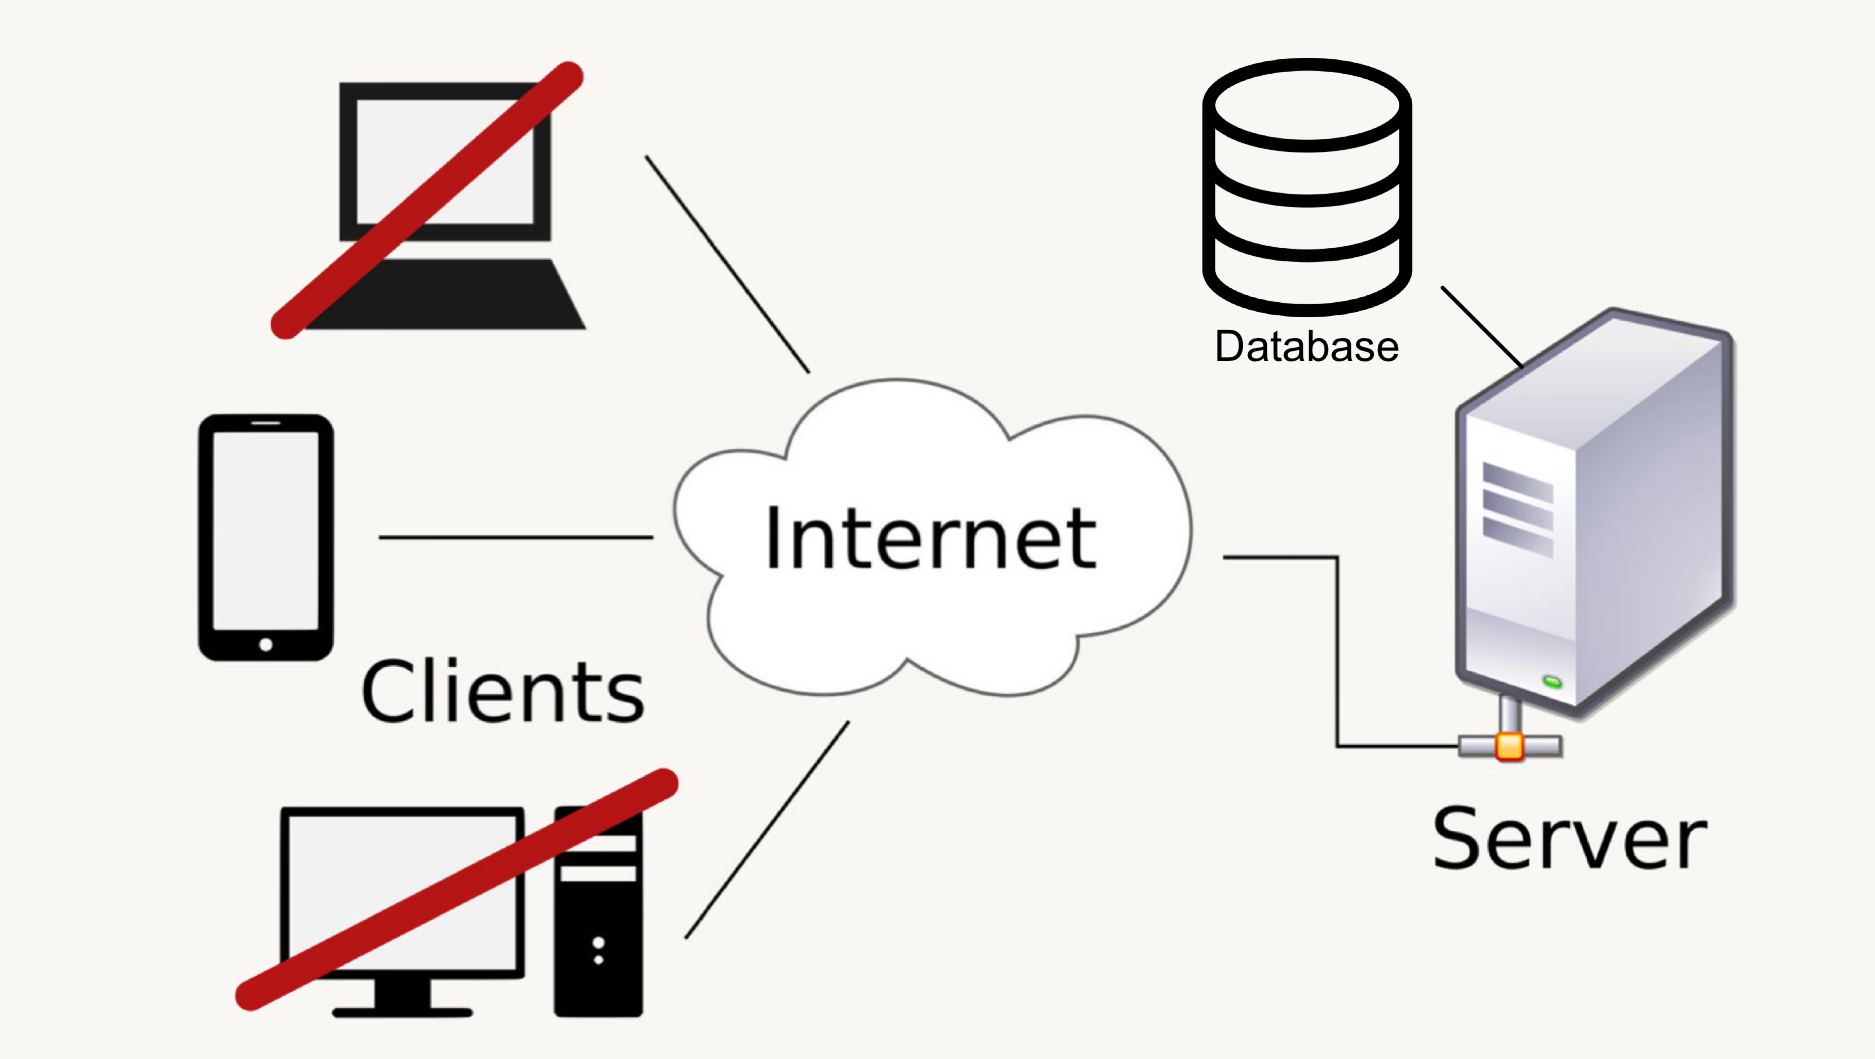
\includegraphics[scale=0.2]{images/high-level-system-architecture.jpg}
  \end{center}
  \caption{High-level software architecture}
  \label{fig:software-archi}
  \source{https://commons.wikimedia.org/wiki/File:Client-server-model.svg (modified by Kendra Birringer)}
\end{figure}
%==============================================================================
\section{Backlog Items}
Backlog items are part of a product backlog. This is an ordered list of requirements which have to be satisfied according to the DoD for the product. The purpose of a backlog item is to take a requirement description, in form of a use case description, as input and build an analysis model of our software capability as result.

We used the \emph{Volere Requirements Specification Template} \cite{volere} also known as \emph{Volere Snow Cards}  as a template to create a list of backlog items using Google Sheets where we collected all of our backlog items.

% This requirement matrix is shown in figure \ref{fig:reqmatrix}.
This requirement matrix is shown below.

% \begin{figure} [htbp]
% \label{fig:reqmatrix}
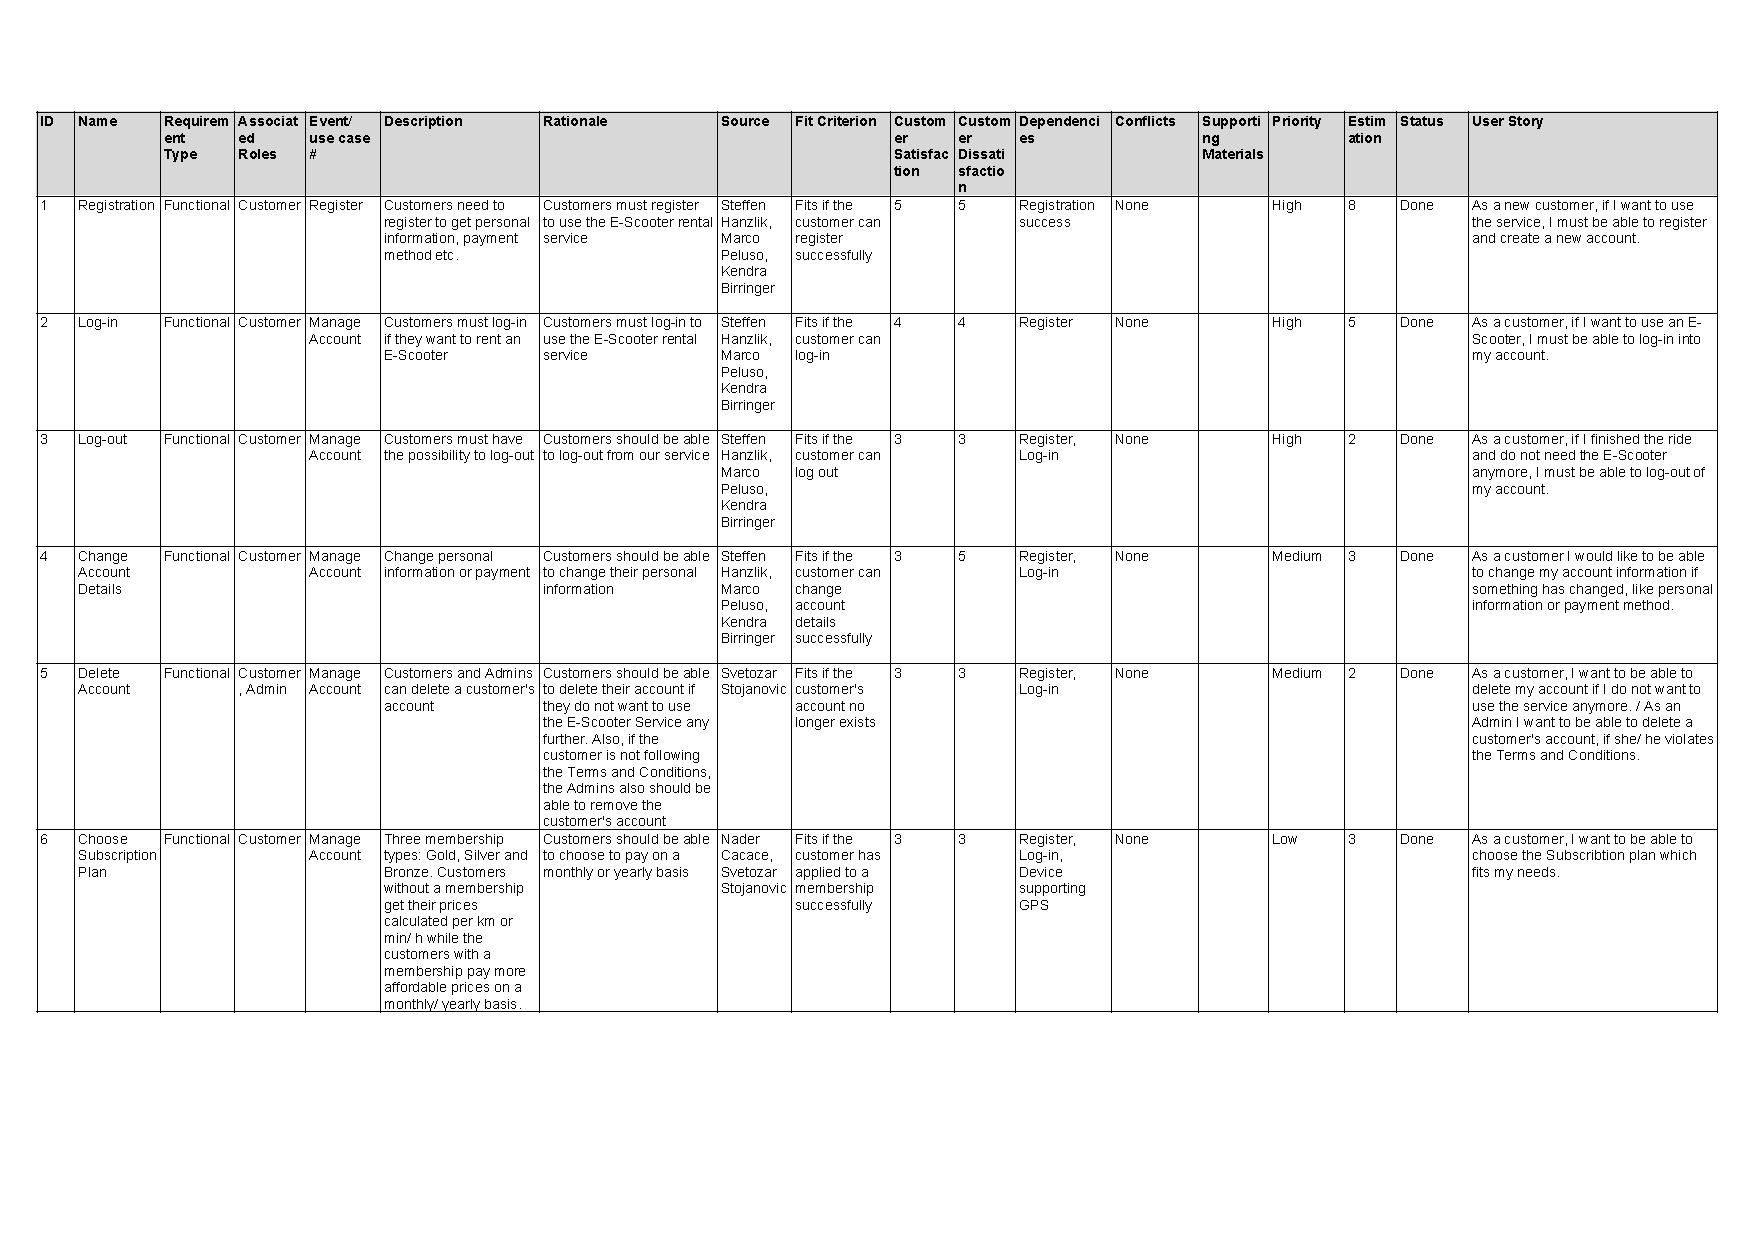
\includepdf[pages=-]{includes/pdf/project-requirements-matrix - BacklogItems.pdf}
% \end{figure}
%==============================================================================
\section{Week One}
%==============================================================================
In the first week a few of our team members rented an E-Scooter from the company "Lime" to gain a better understanding of the process of renting an E-Scooter. That really helped us to find additional requirements for our E-Scooter rental service project. As we already mentioned before, we collected those requirements in a Google Sheets document. That way we could easily collaborate on them, even if we sometimes could not meet at the same location. We also started to talk about the requirements' estimations, satisfactions conditions, priorities, and fit criteria.

The estimation of the effort required to complete the backlog items, was difficult for our team, since we were all inexperienced in that regard. That's why we decided to play "Planning Poker", which is "[\ldots] a consensus-based estimating technique. Agile teams around the world use Planning Poker to estimate their product backlogs. Planning Poker can be used with story points, ideal days, or any other estimating unit." \cite{planning-poker} This proved to be very helpful and was also a lot of fun for our team.

We mostly spent the rest of the week with the collection of more requirements for the project.

Since our team members had vastly different schedules, finding dates for further meetings turned out to be very difficult. That lead us to the decision to have regular weekly instead of daily meetings and whenever there would occur any problems which needed to be discussed, via "Discord". Discord is an "All-in-one voice and text chat [\ldots] that's free, secure, and works on both your desktop and phone."\cite{discord}

\subsection{Division of Work: Week One}
\begin{table}[htbp]
\centering
\setlength{\tabcolsep}{10pt}
\begin{tabular}{|c|c|c|c|c|}
\hline
K. Birringer & N. Cacace & S. Hanzlik & M. Peluso & S. Stojanovic\\
\hline
20\%   &20\%  &20\%  &20\%  &20\%\\
\hline
\end{tabular}
\end{table}
%==============================================================================
\section{Week Two}
%==============================================================================
Since we decided to use the agile method Scrum for analyzing the E-Scooter rental service project, the team members were assigned the following roles:

\begin{itemize}
\item Development Team: Kendra Birringer, Nader Cacace, Steffen Hanzlik,\\
      Marco Peluso, Svetozar Stojanovic
      
The Development Team was responsible for modeling all neccessary UML diagrams and sketching UI prototypes.

\item Scrum Master: Kendra Birringer

In addition to her role as a member of the development team, Kendra also took on the role of the Scrum Master. She was responsible for the organization of the whole team: she organized and moderated the team meetings and wrote the protocols. 

Another task was to check and correct the spelling, grammar and contents of everything that was written.

\item Tester: Marco Peluso

Marco also acted as the tester. He mainly reviewed, documented and accepted the resulting artifacts.
\end{itemize}

In the second week the team discussed each of the collected requirements, and we decided which of them fit and which are not necessary for the software. During this discussion we gathered more requirements.

Then we started to talk about the UML diagrams and built a first use case diagram which was too big and complex and needed some adjustments. So, the task for the Development Team was to simplify the diagram and make it clearer. Our solution for this problem was to build smaller use case diagrams in addition to the big overview, that just display a single use case in each of them (see Appendix). This was done by Kendra, Svetozar and Marco.

Also, Kendra, Marco and Steffen built a main structure for the documentation of the project and started writing the documentation with LaTex. 

\subsection{Division of Work: Week Two}
\begin{table}[htbp]
\centering
\setlength{\tabcolsep}{10pt}
\begin{tabular}{|c|c|c|c|c|}
\hline
K. Birringer & N. Cacace & S. Hanzlik & M. Peluso & S. Stojanovic\\
\hline
18\%   &21\%  &22\%  &18\%  &21\%\\
\hline
\end{tabular}
\end{table}

%==============================================================================
\section{Week Three}
%===============================================================================
In week three the Development Team modified the use case diagram which was too big. They also modeled further use case diagrams which we then discussed, to find out if they needed further adjustments. At the end of this week, we finished the use case diagrams and Kendra finally added the use case documentation to each use case.

Also, after we thought about where it could be necessary, some activity and sequence diagrams were modeled.

Steffen and Kendra started modeling the following activity diagrams: 
\begin{itemize}
    \item Check-in E-Scooter
    \item Check-out E-Scooter
    \item Log-in
    \item Log-out
    \item Manage Account
    \item Register
\end{itemize}


Svetozar and Marco modeled the following activity diagrams:
\begin{itemize}
    \item Give Feedback
    \item Pay the Service
    \item Report problems with the Scooter
\end{itemize}

Nader worked on the following sequence diagrams:
\begin{itemize}
    \item Check-in E-Scooter
    \item Check-out E-Scooter
    \item Add E-Scooter to System
    \item Find an E-Scooter on the Map
    \item Reserve an E-Scooter
    \item Register
    \item Report Problems with the Scooter
\end{itemize}

Marco reviewed Nader's sequence diagrams and did some tweaks and adjustments to them.

Also, Svetozar and Marco worked on the Wallet Management sequence diagram.

Then we started to think about the class diagram and asked ourselves which classes we needed and which relations the different classes could have to each other. Then Steffen and Marco started modeling the class diagram.

Furthermore, the first UI prototype "Start Menu" was built with the software design tool \emph{Axure} \cite{axure}.  This was mainly done by Svetozar. 

\subsection{Division of Work: Week Three}
\begin{table}[htbp]
\centering
\setlength{\tabcolsep}{10pt}
\begin{tabular}{|c|c|c|c|c|}
\hline
K. Birringer & N. Cacace & S. Hanzlik & M. Peluso & S. Stojanovic\\
\hline
19\%   &12\%  &25\%  &19\%  &25\%\\
\hline
\end{tabular}
\end{table}

%==============================================================================
\section{Week Four}
%===============================================================================
During week four we refined the state of the project by doing a lot of adjustments and modifications to everything we had done so far. We updated the requirements, Kendra checked the spelling and grammar, put the requirements in a proper order and Marco checked what was still missing and controlled and adjusted all of the diagrams which needed further improvements.

On the basis of the backlog items list we finished all UML diagrams and Svetozar finished all UI prototypes (see Appendix).
After we heard the lecture, in which Prof. Dr.-Ing Peter Thoma talked about UML diagrams, Steffen noticed, that all our activity diagrams lacked a cancellation mode. Therefore, Steffen and Kendra adjusted all these diagrams and added a cancellation mode to them. 

Marco and Kendra finished most of the documentation, so that only the appendices needed to be added.

The goal of our team was, to finish everything until the end of this week, so that in the following week, we would be able to fully concentrate on the presentation of the project.

\subsection{Division of Work: Week Four}

\begin{table}[htbp]
\centering
\setlength{\tabcolsep}{10pt}
\begin{tabular}{|c|c|c|c|c|}
\hline
K. Birringer & N. Cacace & S. Hanzlik & M. Peluso & S. Stojanovic\\
\hline
22\%   &12\%  &21\%  &20\%  &25\%\\
\hline
\end{tabular}
\end{table}

%==============================================================================
\section{Week Five}
%===============================================================================
In week five, we checked everything again and finished everything.
Kendra generated the use case report from MagicDraw. Because the smaller use cases were not included in the report, you can find them in the Appendix.

Also all team meeting protocols were added by Marco and Kendra.

The user interface prototypes were added as screenshots to the appendix to the project's documentation.

Once the documentation was finished, each team member checked it again and made any necessary improvements, corrections and additions.

Then, finally the whole team started to work on preparing the presentation. At first, our presentation was a bit too detailed to fit into the 10 minute time limit, which we found out during our first rehearsal. We trimmed it down bit by bit until we could comfortable perform it under 10 minutes (see Appendix).
%==============================================================================
\subsection{Division of Work: Week Five}

\begin{table}[htbp]
\centering
\setlength{\tabcolsep}{10pt}
\begin{tabular}{|c|c|c|c|c|}
\hline
K. Birringer & N. Cacace & S. Hanzlik & M. Peluso & S. Stojanovic\\
\hline
23\%   &11\%  &20\%  &30\%  &16\%\\
\hline
\end{tabular}
\end{table}


%\newpage
\section{Conclusion}
Despite our team not being able to meet at the same location most of the time, our process did turn out to work quite well. As we already mentioned, we adapted the Scrum framework to our specific needs in terms of meetings, in that we only meet once a week, regularly and used previously mentioned collaboration tools like Discord, Google Sheets and GitHub.


In the middle of the of the project we became a little stuck and could not complete all the sprint items. We had problems with the sequence and activity diagrams. First, we had to do some more research regarding these type of diagrams. This slowed down our workflow and we had to finish a few sprint items a week later, than we had scheduled. Also we had to get familiar with the UI prototyping tools. In the last 3 weeks, we had less problems and worked more to our schedule/planning.

Overall we faced a few problems, but in the end everything was done to the best of our abilities.  This experience was really educational for this project and our further projects. The work could be clearly divided, because of the sprint items and everybody always knew what they had to do. Communication between the team members worked very well due to the regular meetings and tools we used.

Finally, this project was one of the biggest projects in our studies so far and we learned a lot. We are very grateful that we had this experience.


%==============================================================================
%\newpage
\section{Appendix}

\includepdf[pagecommand={\subsection{Use Case Report}}]{includes/pdf/UseCase_Report.pdf}

\includepdf[pages=2-]{includes/pdf/UseCase_Report.pdf}
%==============================================================================
\subsection{Detailed Use Case Diagrams}
\begin{figure} [htbp]
  \begin{center}
    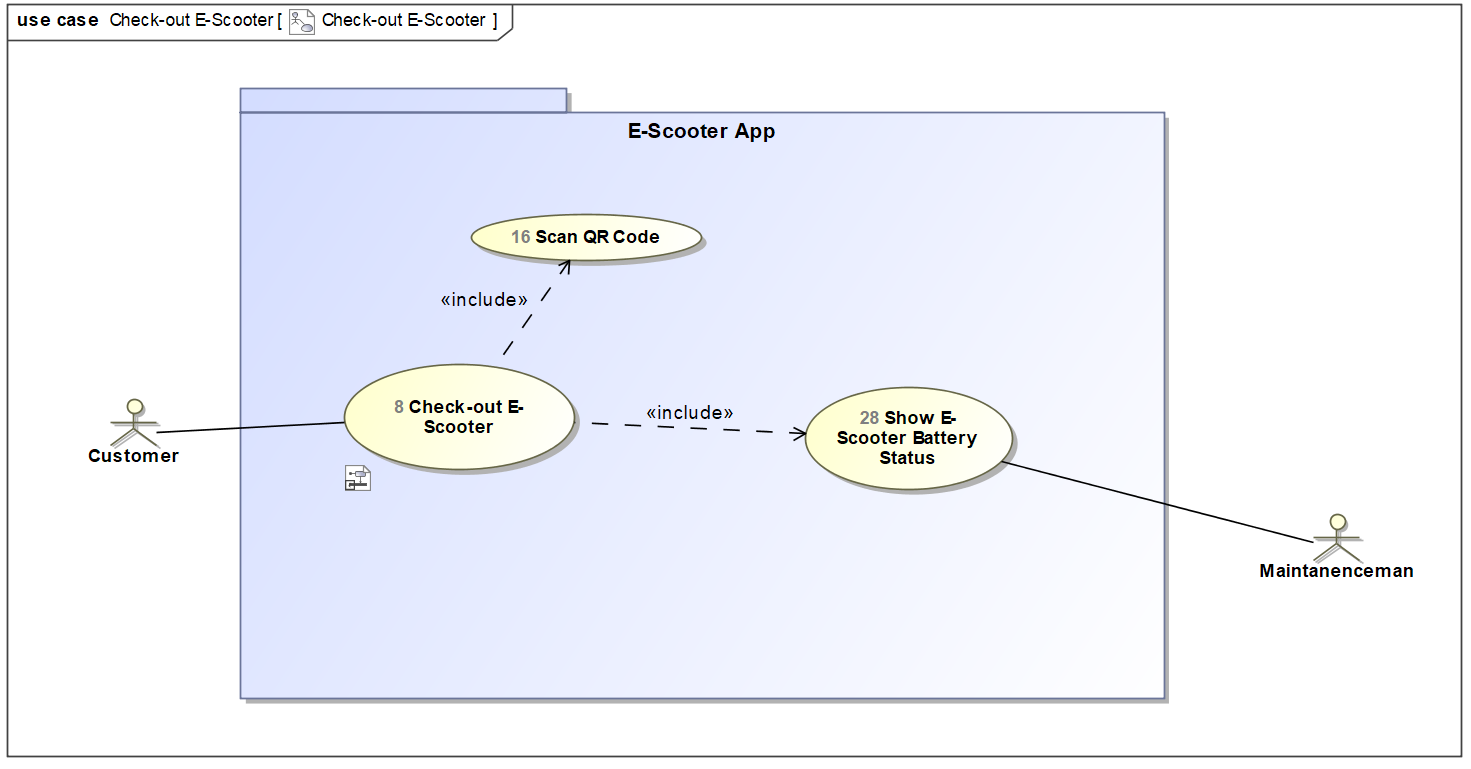
\includegraphics[scale=0.52]{images/UseCases/Check-OutE-Scooter.png}
  \end{center}
  \caption{Use Case: Check-Out E-Scooter}
\end{figure}

\begin{figure} [htbp]
  \begin{center}
    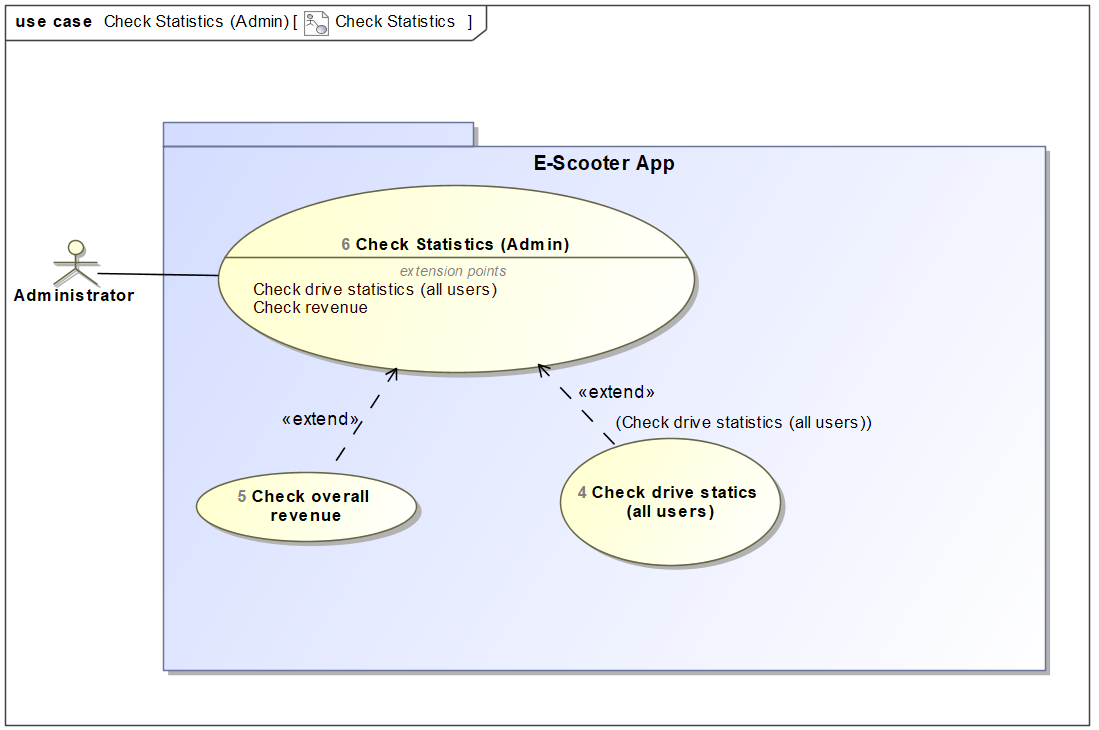
\includegraphics[scale=0.7]{images/UseCases/CheckStatistics(Admin).png}
  \end{center}
  \caption{Use Case: Check Statistics (Admin)}
\end{figure}

\begin{figure} [htbp]
  \begin{center}
    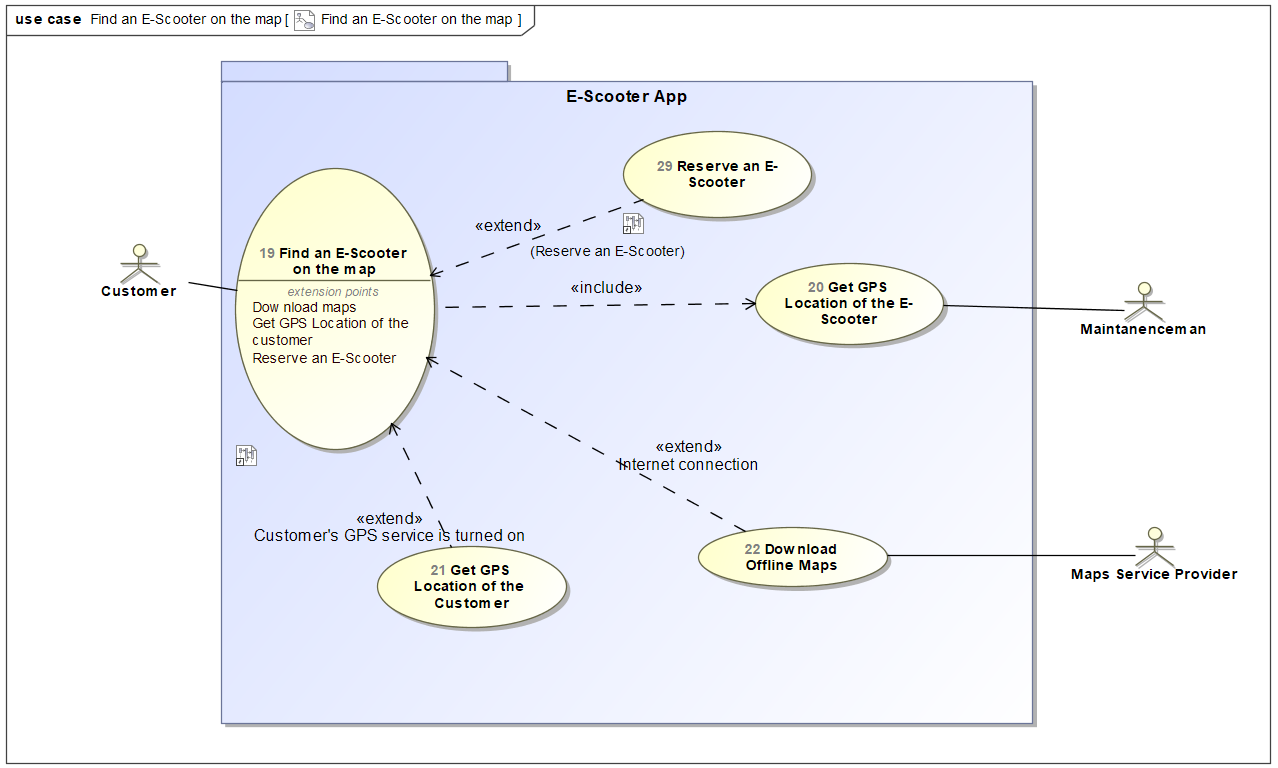
\includegraphics[scale=0.6]{images/UseCases/FindE-ScooterOnTheMap.png}
  \end{center}
  \caption{Use Case: Find an E-Scooter on the map}
\end{figure}

\begin{figure} [htbp]
  \begin{center}
    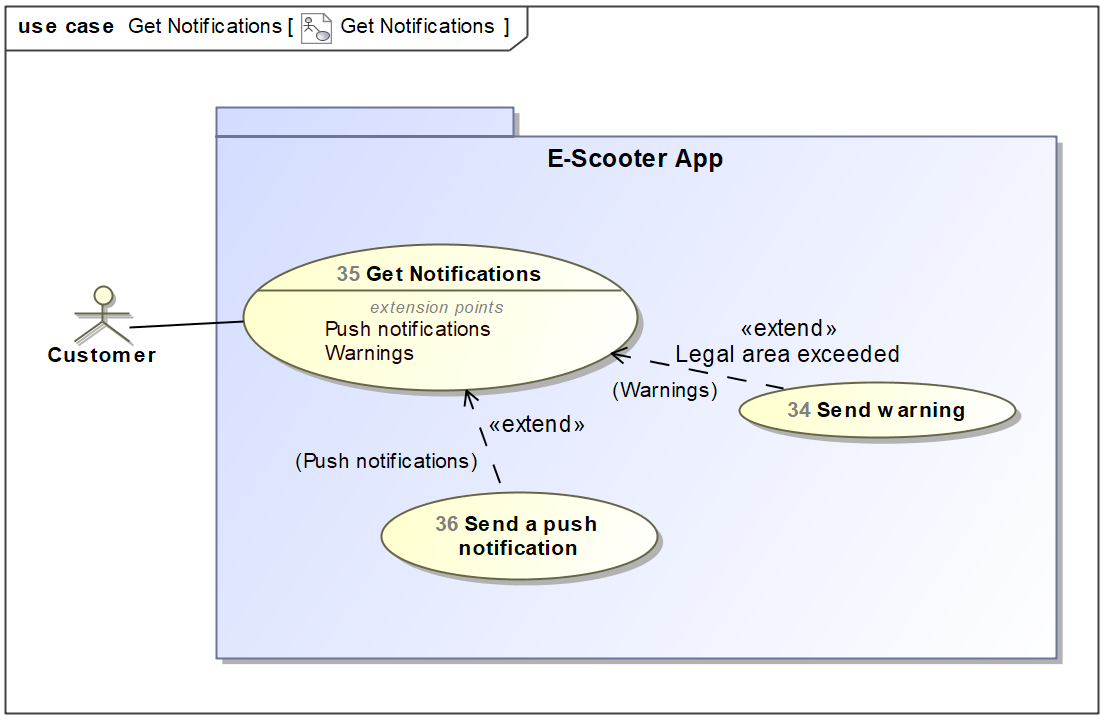
\includegraphics[scale=0.6]{images/UseCases/GetNotifications.png}
  \end{center}
  \caption{Use Case: Get Notifications}
\end{figure}

\begin{figure} [htbp]
  \begin{center}
    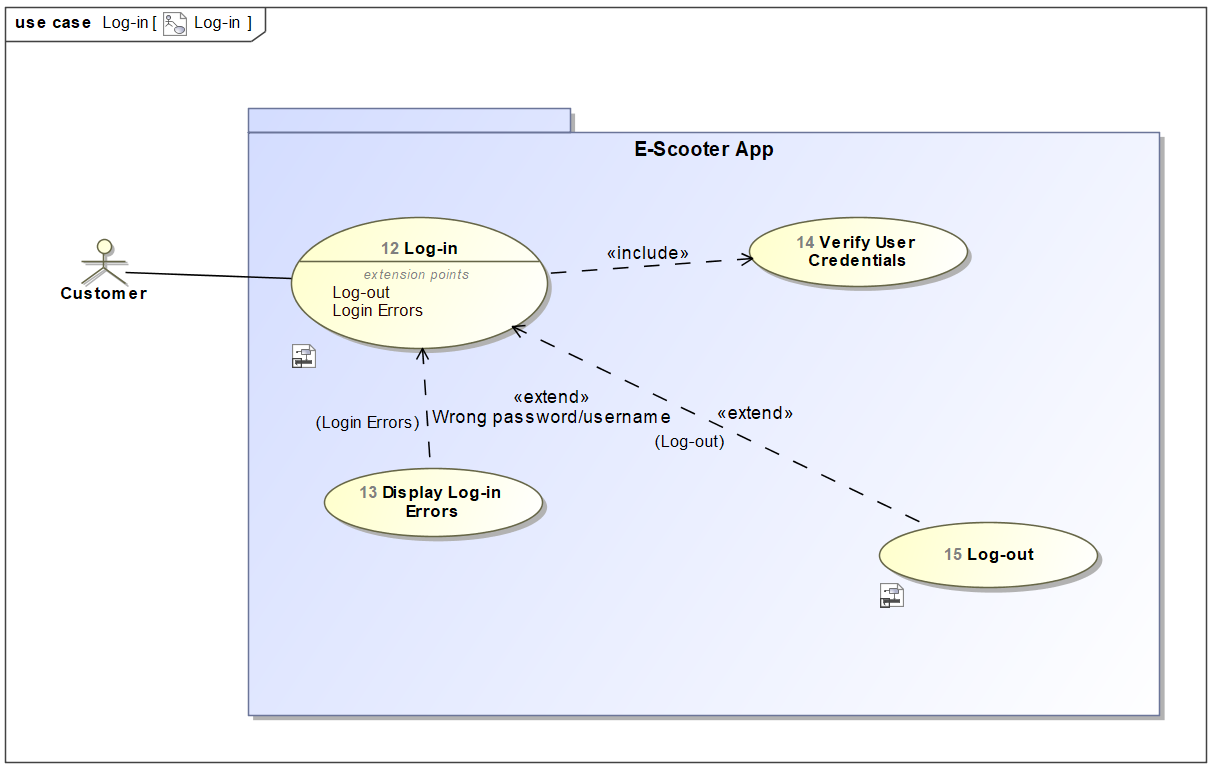
\includegraphics[scale=0.6]{images/UseCases/Log-in.png}
  \end{center}
  \caption{Use Case: Log-in}
\end{figure}

\begin{figure} [htbp]
  \begin{center}
    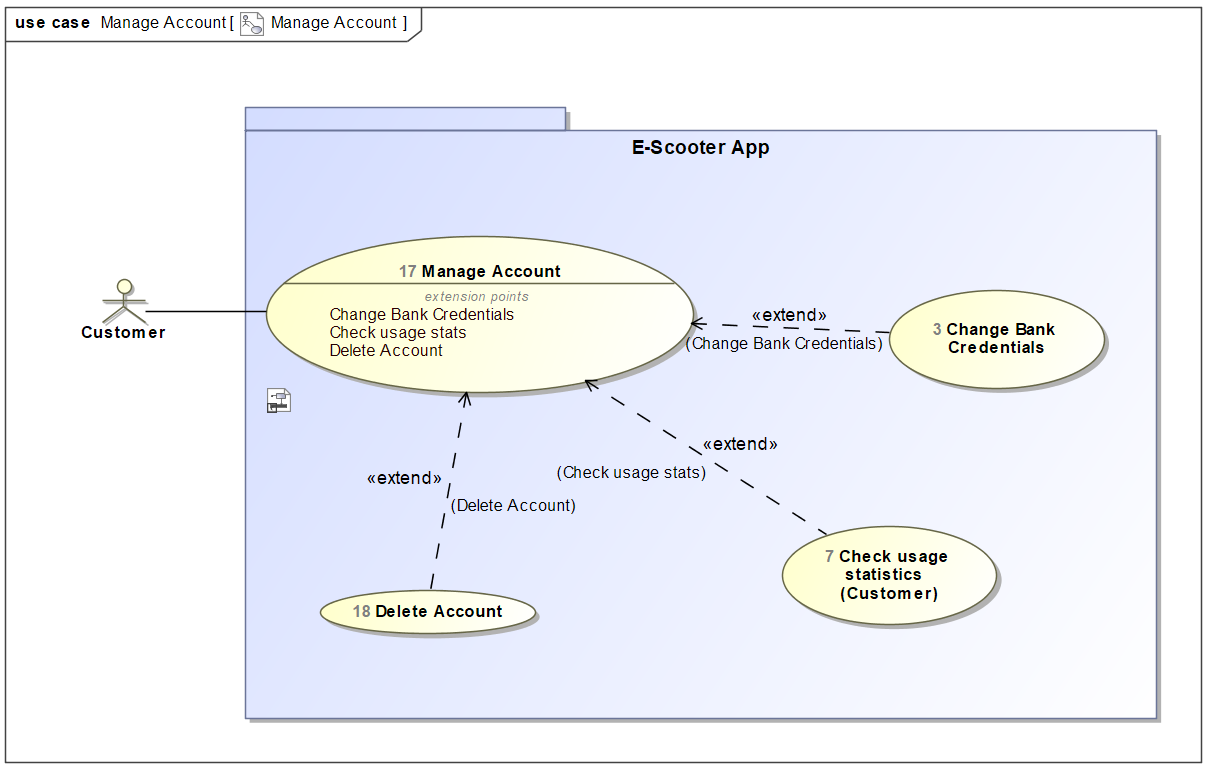
\includegraphics[scale=0.6]{images/UseCases/ManageAccount.png}
  \end{center}
  \caption{Use Case: Manage Account}
\end{figure}

\begin{figure} [htbp]
  \begin{center}
    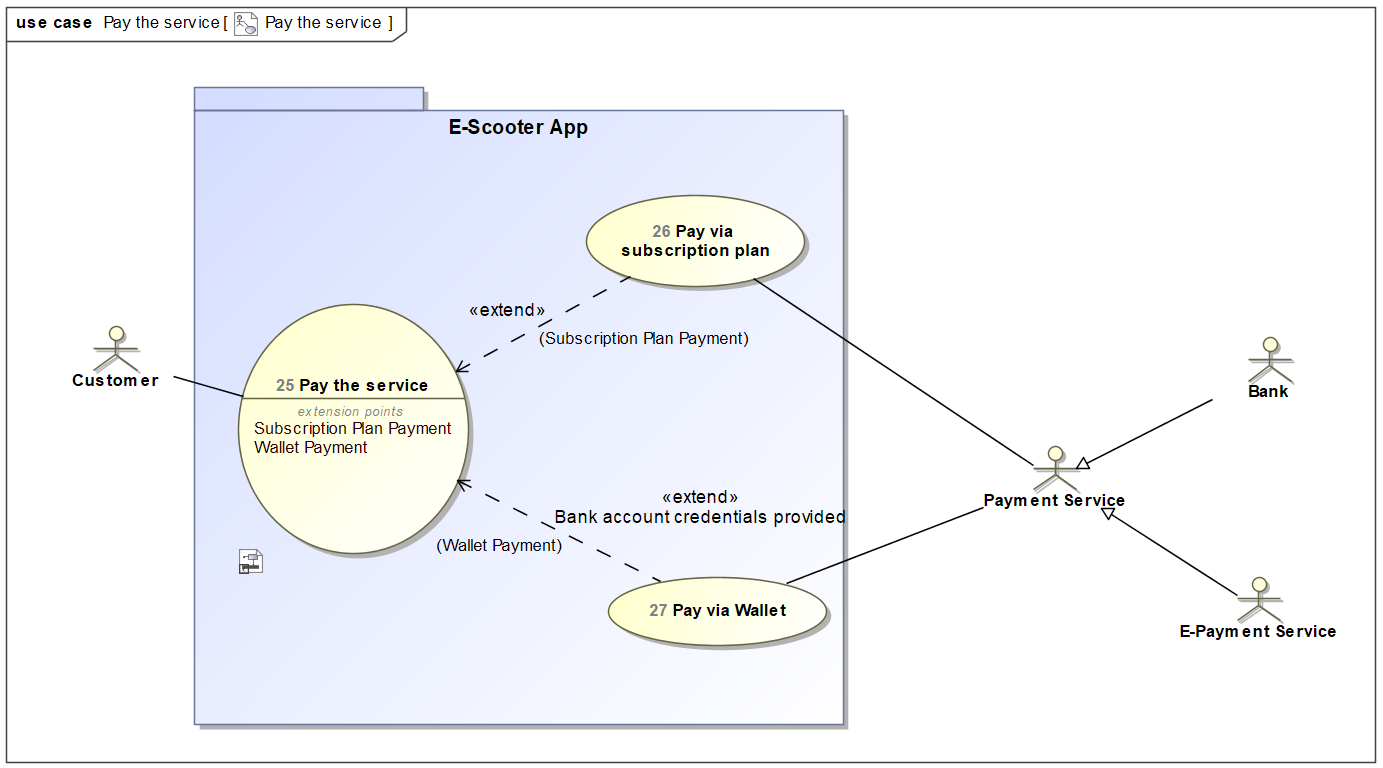
\includegraphics[scale=0.58]{images/UseCases/PayTheService.png}
  \end{center}
  \caption{Use Case: Pay The Service}
\end{figure}

\begin{figure} [htbp]
  \begin{center}
    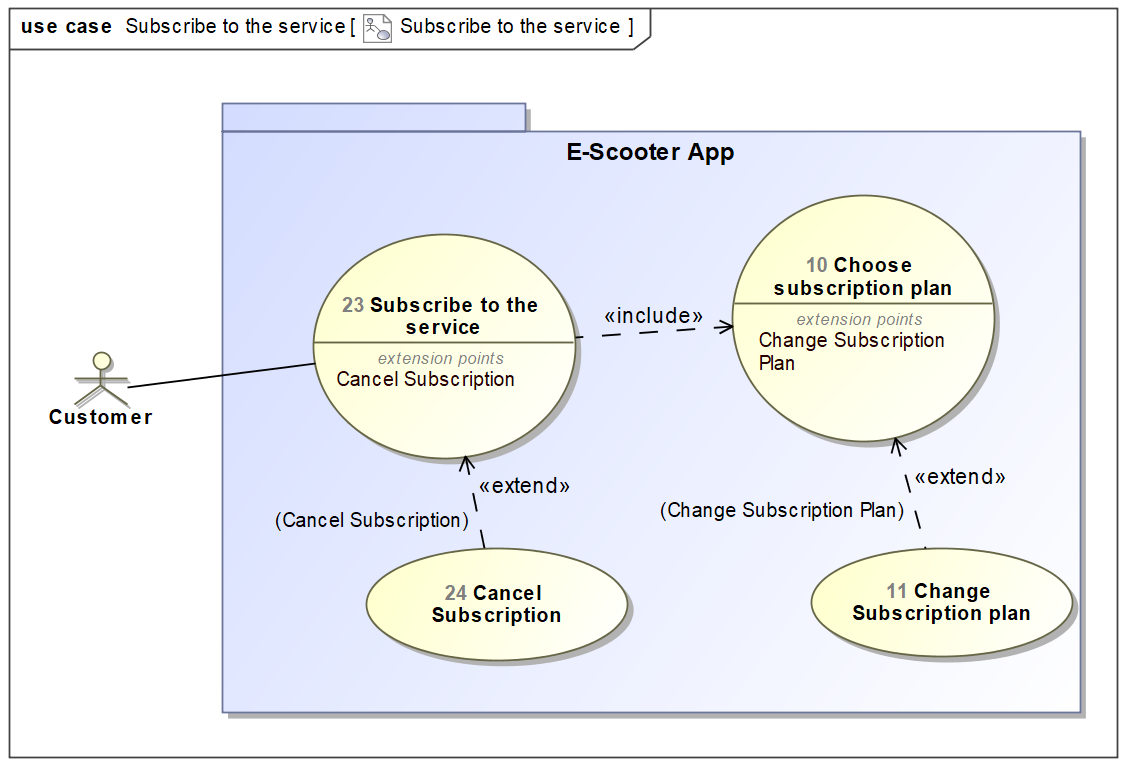
\includegraphics[scale=0.7]{images/UseCases/SubscribeToTheService.png}
  \end{center}
  \caption{Use Case: Subscribe to The Service}
\end{figure}



%==============================================================================
\newpage
\subsection{Class Diagram}
  \begin{center}
    \includegraphics[scale=0.37,angle=90,origin=c]{images/class-diagram.png}
  \end{center}
  
%==============================================================================
\newpage

\includepdf[pagecommand={\subsection{Presentation Slides}}]{includes/pdf/presentation.pdf}

\includepdf[pages=2-]{includes/pdf/presentation.pdf}
%==============================================================================
\newpage
\subsection{UI Prototypes}

\begin{figure} [htbp]
    \begin{center}
        \begin{minipage}{0.45\textwidth}
            \begin{center}
                 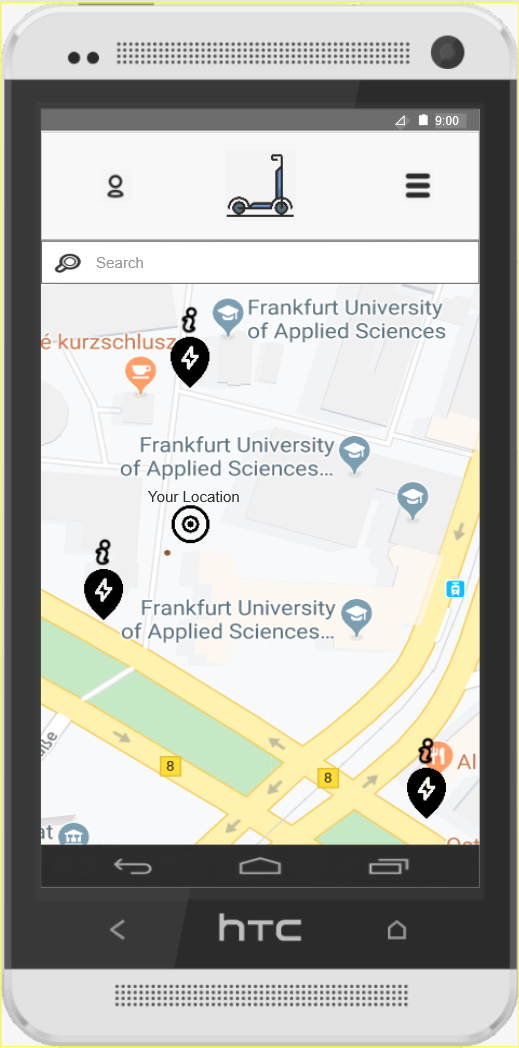
\includegraphics[scale=0.65]{images/prototypes/01-start-menu.png}
            \end{center}
            \caption{Start Menu}
        \end{minipage}\hfill
        \begin{minipage}{0.45\textwidth}
            \begin{center}
                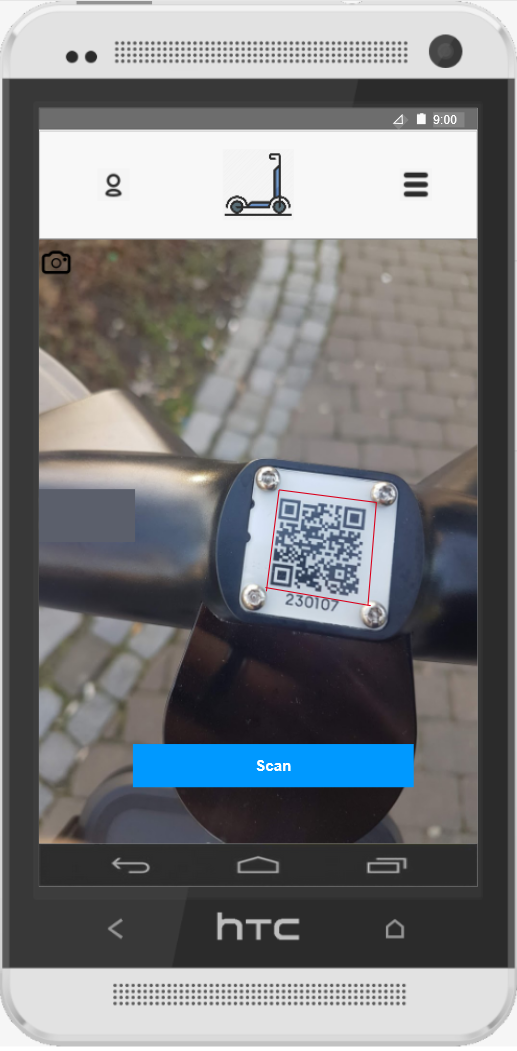
\includegraphics[width=0.87\textwidth]{images/prototypes/01-01-start-menu--scan-qr-code.png}
            \end{center}
            \caption{Start Menu $\rightarrow$ Scan QR-Code}
        \end{minipage}
    \end{center}
\end{figure}

\begin{figure} [htbp]
    \begin{center}
        \begin{minipage}{0.45\textwidth}
            \begin{center}
                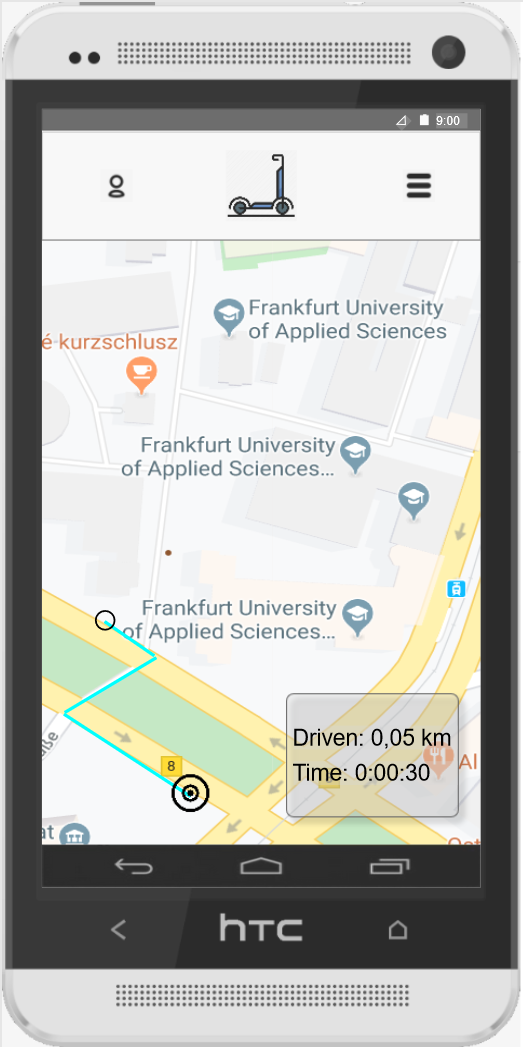
\includegraphics[scale=0.65]{images/prototypes/01-02-start-menu---driving.png}
            \end{center}
            \caption{Start Menu $\rightarrow$ Driving}
        \end{minipage}\hfill
        \begin{minipage}{0.45\textwidth}
            \begin{center}
                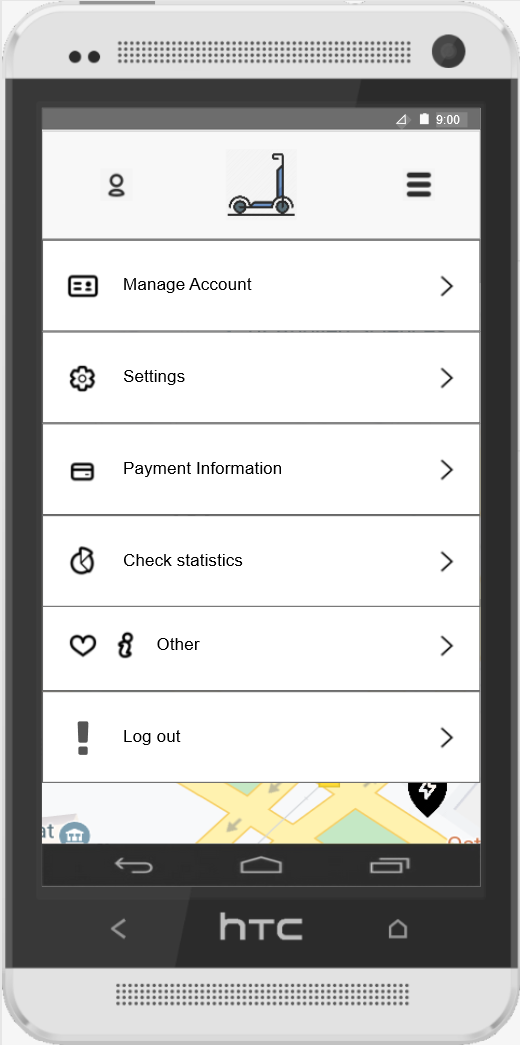
\includegraphics[scale=0.65]{images/prototypes/02-menu-dropdown.png}
            \end{center}
            \caption{Menu Dropdown}
        \end{minipage}
    \end{center}
\end{figure}


\begin{figure} [htbp]
    \begin{center}
        \begin{minipage}{0.45\textwidth}
            \begin{center}
                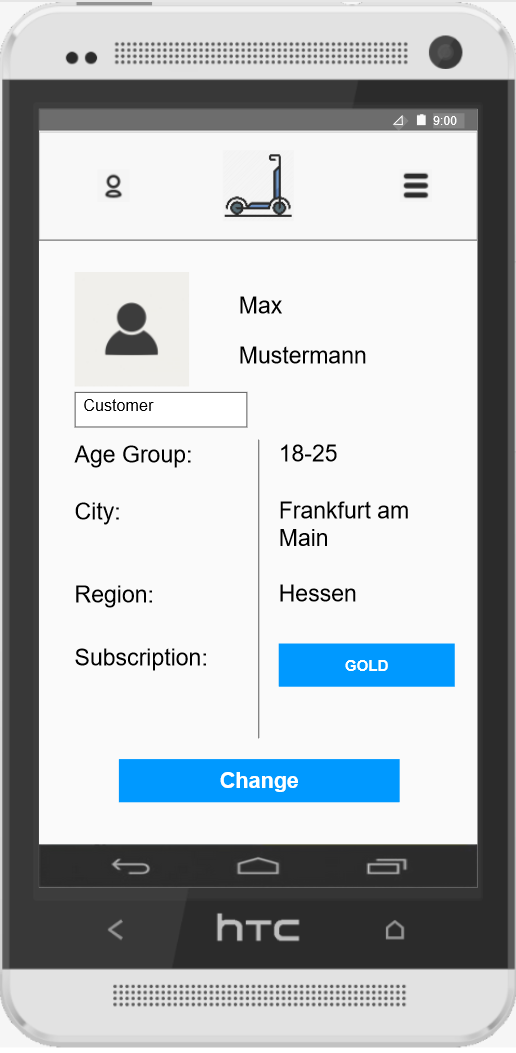
\includegraphics[scale=0.65]{images/prototypes/02-01-menu-dropdown--account-management.png}
            \end{center}
            \caption{Menu Dropdown $\rightarrow$ Account Management}
        \end{minipage}\hfill
        \begin{minipage}{0.45\textwidth}
            \begin{center}
                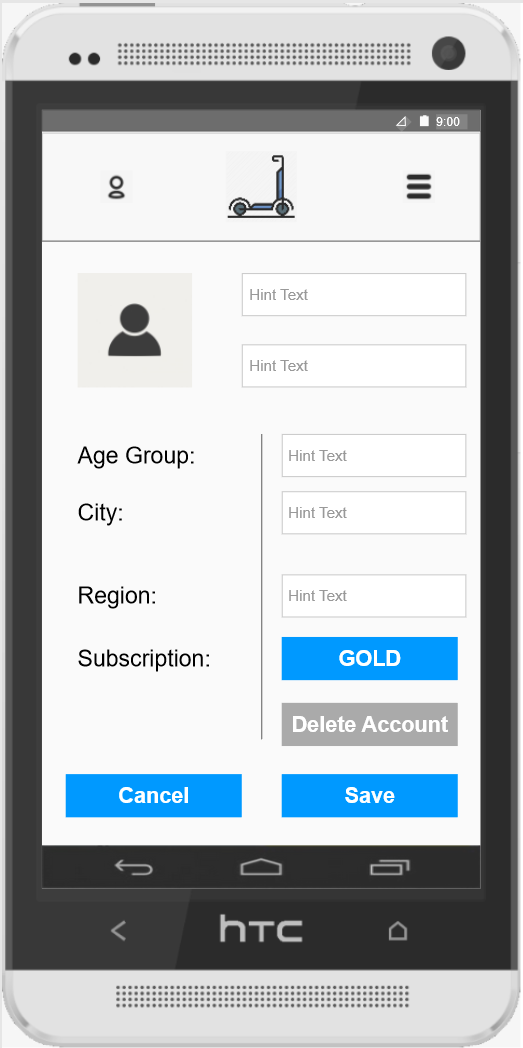
\includegraphics[scale=0.65]{images/prototypes/02-01-01-menu-dropdown--account-management--change-account-details.png}
            \end{center}
            \caption{Menu Dropdown $\rightarrow$ Account Management $\rightarrow$ Change Account Details}
        \end{minipage}
    \end{center}
\end{figure}

\begin{figure} [htbp]
    \begin{center}
        \begin{minipage}{0.45\textwidth}
            \begin{center}
                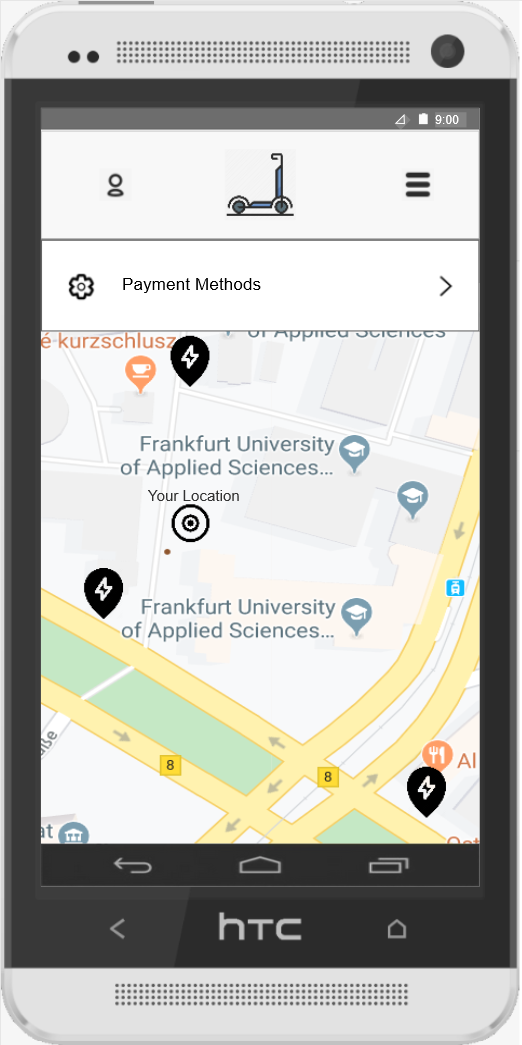
\includegraphics[scale=0.65]{images/prototypes/02-02-menu-dropdown--payment-information.png}
            \end{center}
            \caption{Menu Dropdown $\rightarrow$ Payment Information}
        \end{minipage}\hfill
        \begin{minipage}{0.45\textwidth}
            \begin{center}
                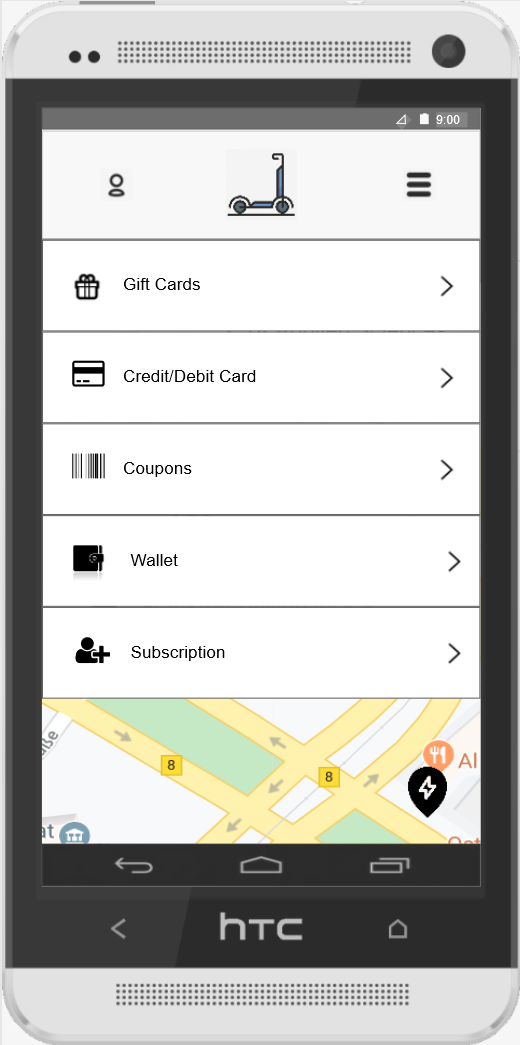
\includegraphics[scale=0.65]{images/prototypes/02-02-01-menu-dropdown--payment-information--payment-methods.png}
            \end{center}
            \caption{Menu Dropdown $\rightarrow$ Payment Information $\rightarrow$ Payment Methods}
        \end{minipage}
    \end{center}
\end{figure}

\begin{figure} [htbp]
    \begin{center}
        \begin{minipage}{0.45\textwidth}
            \begin{center}
                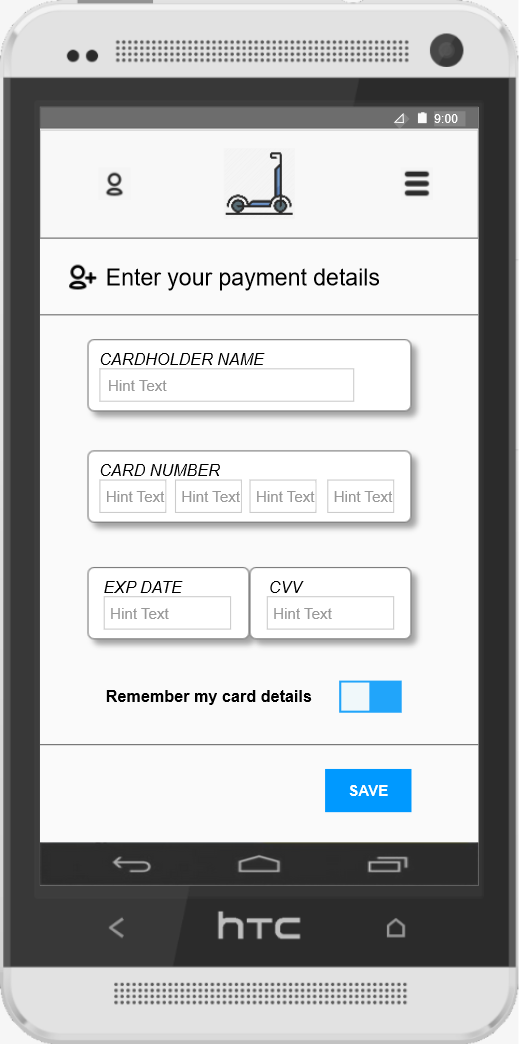
\includegraphics[scale=0.65]{images/prototypes/02-02-01-01-menu-dropdown--payment-information--payment-methods--credit-debit-card-info.png}
            \end{center}
            \caption{Menu Dropdown $\rightarrow$ Payment Information $\rightarrow$ Payment Methods $\rightarrow$ Credit/Debit Card}
        \end{minipage}\hfill
        \begin{minipage}{0.45\textwidth}
            \begin{center}
                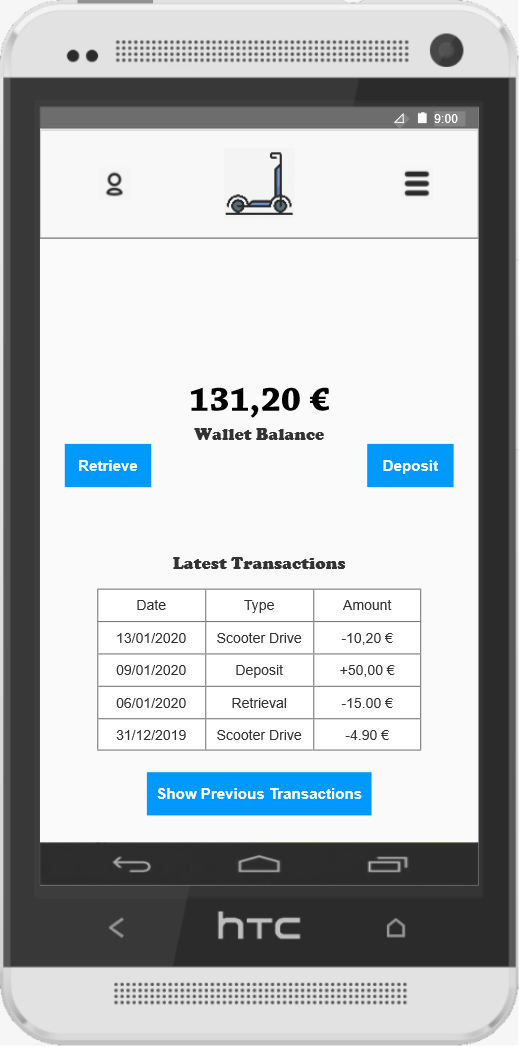
\includegraphics[scale=0.65]{images/prototypes/02-02-01-02-menu-dropdown--payment-information--payment-methods--wallet.png}
            \end{center}
            \caption{Menu Dropdown $\rightarrow$ Payment Information $\rightarrow$ Payment Methods $\rightarrow$ Wallet}
        \end{minipage}
    \end{center}
\end{figure}

\begin{figure} [htbp]
    \begin{center}
        \begin{minipage}{0.45\textwidth}
            \begin{center}
                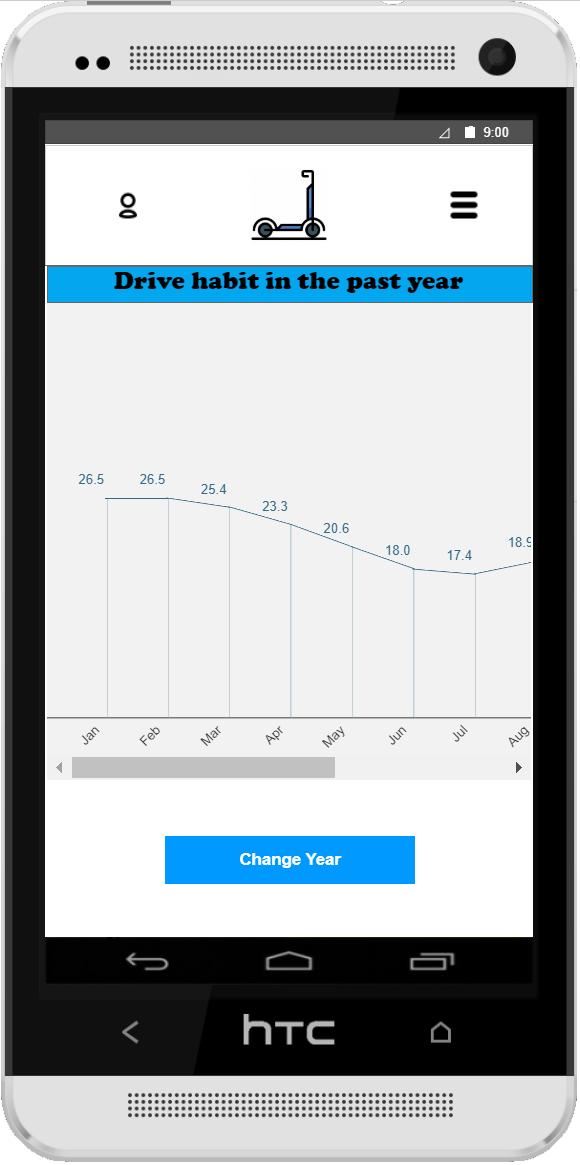
\includegraphics[scale=0.59]{images/prototypes/02-03-menu-dropdown--check-drive-statistics.png}
            \end{center}
            \caption{Menu Dropdown $\rightarrow$ Check Drive Statistics}
        \end{minipage}\hfill
        \begin{minipage}{0.45\textwidth}
            \begin{center}
                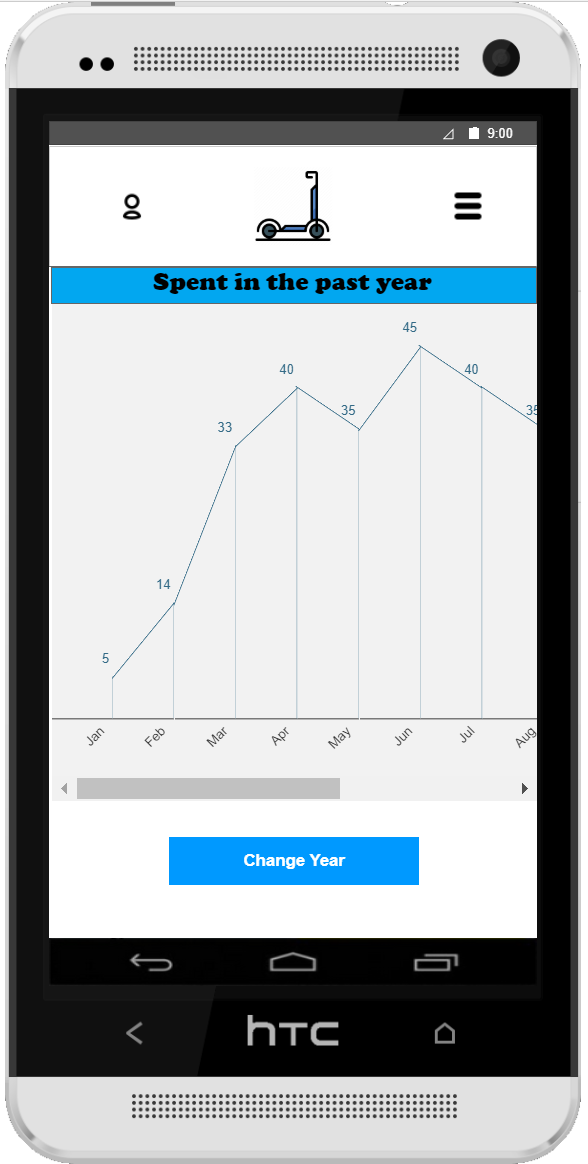
\includegraphics[scale=0.59]{images/prototypes/02-04-menu-dropdown--check-spent-money.png}
            \end{center}
            \caption{Menu Dropdown $\rightarrow$ Check Spent Money}
        \end{minipage}
    \end{center}
\end{figure}

\begin{figure} [htbp]
    \begin{center}
        \begin{minipage}{0.45\textwidth}
            \begin{center}
                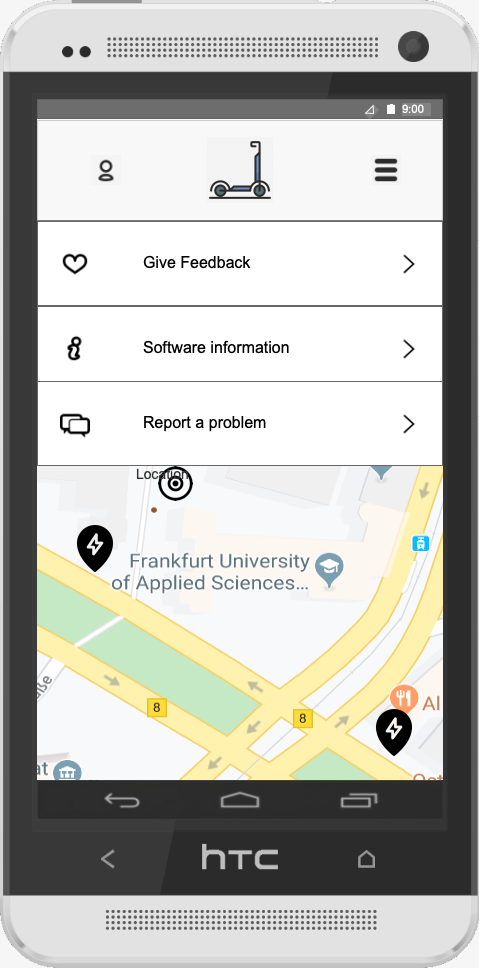
\includegraphics[scale=0.35]{images/prototypes/02-05-menu-dropdown--other.png}
            \end{center}
            \caption{Menu Dropdown $\rightarrow$ Other}
        \end{minipage}\hfill
        \begin{minipage}{0.45\textwidth}
            \begin{center}
                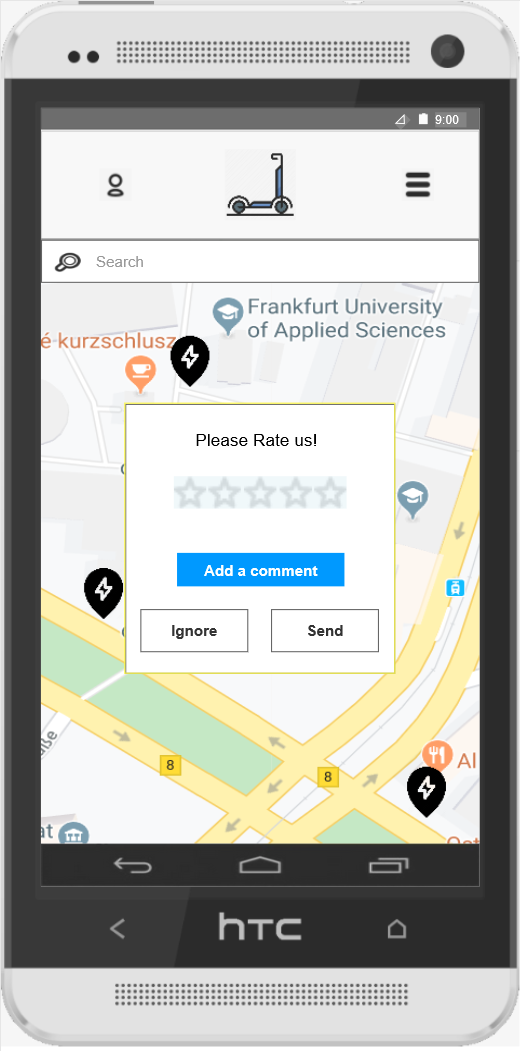
\includegraphics[scale=0.65]{images/prototypes/03-ask-for-feedback.png}
            \end{center}
            \caption{Ask for Feedback}
        \end{minipage}
    \end{center}
\end{figure}

\begin{figure} [htbp]
    \begin{center}
        \begin{minipage}{0.45\textwidth}
            \begin{center}
                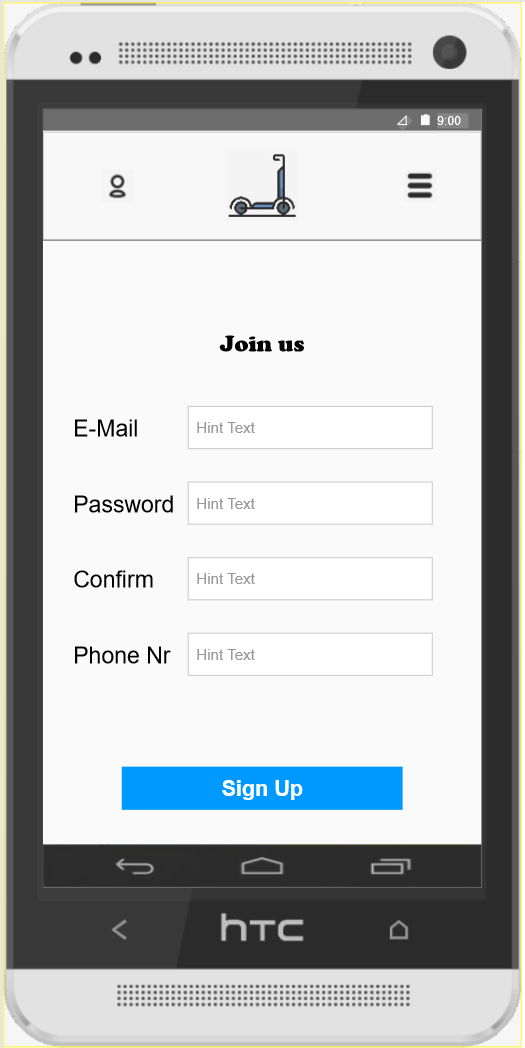
\includegraphics[scale=0.65]{images/prototypes/04-register-sign-up.png}
            \end{center}
            \caption{Register/Sign Up}
        \end{minipage}\hfill
        \begin{minipage}{0.45\textwidth}
            \begin{center}
                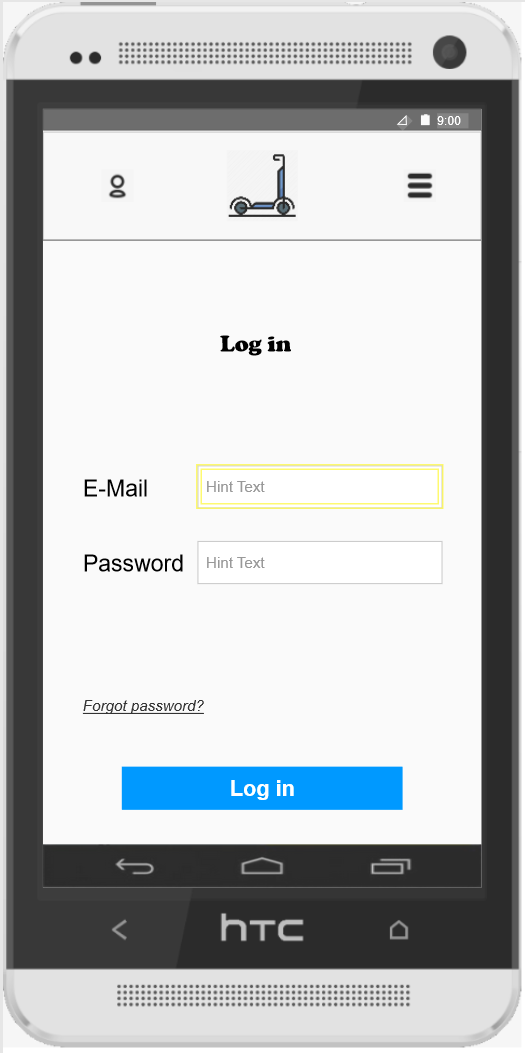
\includegraphics[scale=0.65]{images/prototypes/05-log-in.png}
            \end{center}
            \caption{Log in}
        \end{minipage}
    \end{center}
\end{figure}

\begin{figure} [htbp]
  \begin{center}
    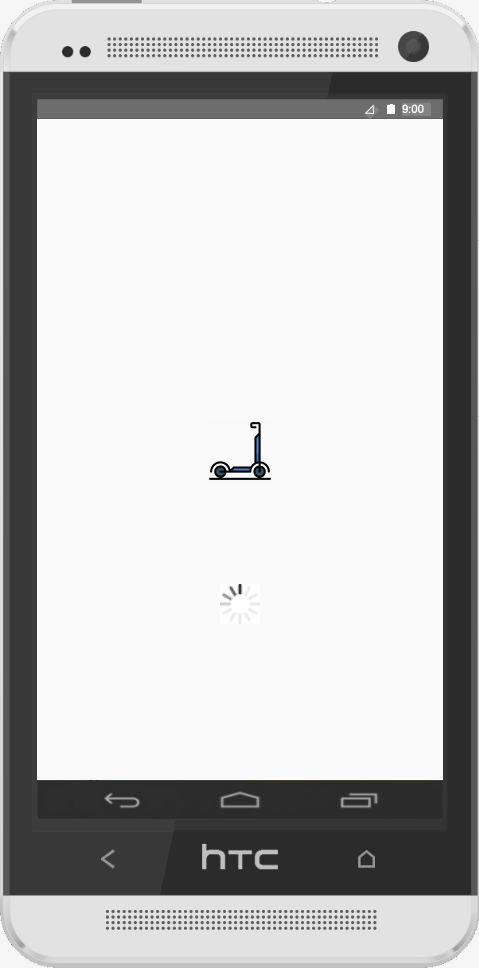
\includegraphics[scale=0.65]{images/prototypes/06-loading-screen.png}
  \end{center}
  \caption{Loading Screen}
\end{figure}
%==============================================================================
\newpage
\subsection{Meeting Protocols}

\protocolheader{Weekly Scrum (Discord)}{1}{2019-12-22}{11:00 - 12:50}
    {Kendra, Nader, Steffen, Marco, Svetozar}
\begin{itemize}
    \item talked about general scope of the project
    \item reviewed some general questions regarding requirements, use cases, prototyping
    \item split up work for the coming week
    \item discussed finding a time slot for daily Scrum meetings, decided to do them weekly instead
    \item confer about structure of the overall system (web-client, app-client, server, ...)
    \item Nader was not sure about requirement \#26
    \item talked about possible roles in our team
    \item intro to git for the less experienced team members
    \item played some planning poker
\end{itemize}

\newpage
\protocolheader{Team Meeting (Café 1)}{1}{2019-12-25}{13:15 - 14:30}
    {Kendra, Steffen, Marco}
\begin{itemize}
    \item set up TexMaker
    \item checked out Overleaf
    \item began to work on LaTeX documentation
    \item reviewed git again
\end{itemize}

\protocolheader{Weekly Scrum (Discord)}{2}{2020-01-19}{11:00 - 12:15}
    {Kendra, Nader, Steffen, Marco, Svetozar}
\begin{itemize}
    \item discussed collected requirements and importance of individual items
    \item shared thoughts about the different kind of uml diagrams
    \item decided to do documentation in LaTeX
    \item split up work into different parts
    \item discuss clean up of big use case diagram
    \item reviewed some of the artifacts according to the DoD
    \item talked about maybe using Trello as Todo-list tool
    \item played some more planning poker, to improve estimations
\end{itemize}

\protocolheader{Weekly Scrum (Discord)}{3}{2020-01-26}{11:00 - 12:30}
    {Kendra, Nader, Steffen, Marco, Svetozar}
\begin{itemize}
    \item reviewed last weeks progress
    \item plan for next week
    \item talked through several backlog items
    \item planning poker again
    \item discussed possible tools for prototyping - Svetozar wanted to try Axure
    \item reviewed some git commands
    \item decided to ditch Trello completely and instead mark backlog items todo status in Google Sheets
    \item talked a lot about uml diagrams
\end{itemize}

\protocolheader{Team Meeting (Café 1)}{3}{2020-01-27}{13:15 - 15:30}
    {Kendra, Steffen, Marco, Svetozar}
\begin{itemize}
    \item tried out a few mockup / prototyping tools (draw.io, balsamiq)
    \item decided to stay with our decision and use Axure
\end{itemize}

\newpage
\protocolheader{Weekly Scrum (Discord)}{4}{2020-02-02}{11:00 - 12:10}
    {Kendra, Nader, Steffen, Marco, Svetozar}
\begin{itemize}
    \item talked about possible improvements of our processes
    \item went over requirements again
    \item reviewed some of the diagrams together and talked about possible improvements
    \item talked about the ui prototypes we wanted to build
    \item set goal to finish everything until end of week, so that we can focus on presentation next week
\end{itemize}

\protocolheader{Weekly Scrum (Discord)}{5}{2020-02-09}{11:00 - 12:10}
    {Kendra, Nader, Steffen, Marco, Svetozar}
\begin{itemize}
    \item reviewed everything we had done so far
    \item discussed about the way we wanted to do the presentation
    \item realized we still have a lot of minor corrections to do in MagicDraw as well as to the documentation, before we could work on presentation - last weeks goal not really reached
\end{itemize}

\protocolheader{Presentation Practice Meeting}{5}{2020-02-07}{11:00 - 12:10}
    {Kendra, Nader, Steffen, Marco, Svetozar}
\begin{itemize}
    \item rehearsed presentation
    \item realized we needed to drastically shorten the presentation
    \item cut a lot of stuff out - decided to give a short overview of everything and then concentrate on a single use case, explaining its different diagrams
    \item rehearsed again a few times and tweaked till we were satisfied with the presentation
\end{itemize}


%==============================================================================
\newpage
\listoffigures

%==============================================================================
\newpage
\begin{thebibliography}{}

\bibitem{scrum}
https://www.scrum.org/resources/what-is-scrum

\bibitem{uml}
https://www.omg.org/spec/UML/

\bibitem{magicdraw}
https://www.nomagic.com/products/magicdraw

\bibitem{thoma}
Prof. Dr.-Ing Peter Thoma \emph{05 Software Engineering Analysis (Software Models and UML)}

\bibitem{axure}
https://www.axure.com/

\bibitem{scrumguide}
https://www.scrumguides.org/scrum-guide.html

\bibitem{thoma1}
Prof. Dr.-Ing Peter Thoma \emph{02-3 Software Engineering Analysis (Scrum)}

\bibitem{volere}
http://www11.informatik.uni-erlangen.de/Lehre/SS2015/PR-SWE/Material/volere-template.pdf

\bibitem{planning-poker}
https://www.mountaingoatsoftware.com/agile/planning-poker

\bibitem{discord}
https://discordapp.com/

\end{thebibliography}
%==============================================================================

\end{document}
